\documentclass[
  a0paper,
  portrait,
  margin=0pt,
  colspace=24pt,
  blockverticalspace=24pt,
  innermargin=40pt,
  fontscale=2.38
]{tikzposter}

\usepackage[T1]{fontenc}
\usepackage[utf8]{inputenc}
\usepackage{amsmath,amssymb}
\usepackage{booktabs}
\usepackage{array}
\usepackage{graphicx}
\usepackage[colalign]{aligncolsatbottom}
\usepackage{helvet}
\usepackage{enumitem}

\renewcommand{\familydefault}{\sfdefault}

\tikzposterlatexaffectionproofoff
\usetikzlibrary{shapes.geometric,arrows.meta,positioning,bending}

\graphicspath{{figures/}}

% -------------------------------------------------
% Optional title logos
% -------------------------------------------------
\newcommand{\titlelogo}{%
  \includegraphics[height=2.8cm]{logo_cs.png}
}
\newcommand{\titlelogoright}{%
  \includegraphics[height=2.2cm]{logo_ps.png}
}
\newlength{\logoleftsep}
\newlength{\logorightsep}
\setlength{\logoleftsep}{1.5cm}
\setlength{\logorightsep}{-1.5cm}

% -------------------------------------------------
% Colors
% -------------------------------------------------
\definecolor{MVAGrey}{gray}{0.93}
\definecolor{MVADark}{gray}{0.15}
\definecolor{MVARed}{RGB}{160,30,45}
\definecolor{PosterSoft}{RGB}{240,243,247}

% -------------------------------------------------
% Theme & Color Style
% -------------------------------------------------
\usetheme{Default}

\definecolorstyle{MVAStyle}{
  \definecolor{ColorOne}{named}{MVADark}
  \definecolor{ColorTwo}{named}{MVARed}
}{
  \colorlet{titlebgcolor}{MVADark}
  \colorlet{titlefgcolor}{white}

  \colorlet{backgroundcolor}{MVAGrey}
  \colorlet{framecolor}{MVADark}

  \colorlet{blocktitlebgcolor}{white}
  \colorlet{blocktitlefgcolor}{ColorTwo!85!black}

  \colorlet{blockbodybgcolor}{white}
  \colorlet{blockbodyfgcolor}{black}

  \colorlet{innerblocktitlebgcolor}{MVAGrey}
  \colorlet{innerblocktitlefgcolor}{ColorTwo!85!black}
  \colorlet{innerblockbodybgcolor}{white}
  \colorlet{innerblockbodyfgcolor}{black}

  \colorlet{notebgcolor}{MVAGrey}
  \colorlet{notefgcolor}{ColorTwo!85!black}
  \colorlet{notefrcolor}{ColorTwo}
}

\usecolorstyle{MVAStyle}

% -------------------------------------------------
% Global spacing tweaks
% -------------------------------------------------
\setlist[itemize]{leftmargin=1.25em,itemsep=0.18em,topsep=0.22em,parsep=0em,partopsep=0em}
\setlist[enumerate]{leftmargin=1.35em,itemsep=0.15em,topsep=0.22em,parsep=0em,partopsep=0em}
\renewcommand{\arraystretch}{1.08}

\AtBeginDocument{
  \setlength{\abovedisplayskip}{0.45em}
  \setlength{\belowdisplayskip}{0.45em}
  \setlength{\abovedisplayshortskip}{0.3em}
  \setlength{\belowdisplayshortskip}{0.3em}
}

% -------------------------------------------------
% Title
% -------------------------------------------------
\title{Warehouse Management with Reinforcement Learning}
\author{Elias Al Bouzidi, Massine El Khader, Idriss Benkirane}

\makeatletter
\renewcommand\TP@maketitle{%
  \begin{tikzpicture}
    \node[inner sep=0pt] at (0,0) {%
      \begin{minipage}{0.12\linewidth}
        \centering
        \titlelogo
      \end{minipage}
      \hspace{\logoleftsep}
      \begin{minipage}{0.74\linewidth}
        \centering
        {\color{titlefgcolor}\bfseries\LARGE \@title \par}
        \vspace{0.30em}


        {\color{titlefgcolor}\large \@author \par}
      \end{minipage}
      \hspace{\logorightsep}
      \begin{minipage}{0.12\linewidth}
        \centering
        \titlelogoright
      \end{minipage}
    };
  \end{tikzpicture}
}
\makeatother

\begin{document}

\renewcommand\normalsize{\fontsize{22}{28}\selectfont}
\renewcommand\small{\fontsize{19}{24}\selectfont}
\renewcommand\footnotesize{\fontsize{17}{22}\selectfont}
\renewcommand\large{\fontsize{26}{32}\selectfont}
\renewcommand\Large{\fontsize{31}{37}\selectfont}
\renewcommand\LARGE{\fontsize{36}{42}\selectfont}

\maketitle[width=0.97\linewidth,titletoblockverticalspace=28pt,linewidth=0,roundedcorners=20]

\begin{columns}

% =================================================
% LEFT COLUMN
% =================================================
\column{0.33}

\block[titleleft,roundedcorners=16]{1. Context \& Operational Problem}{
\raggedright
\begin{itemize}
\item We study a \textbf{three-warehouse inventory control problem} in a hub-and-spoke logistics network.
\item \textbf{W1} is the central hub, while \textbf{W2} and \textbf{W3} are spoke warehouses with lower capacity and more expensive direct imports.
\item Each month, the controller decides how much to import and whether to transfer stock before stochastic demand is realized.
\item The operational trade-off is between service quality, holding cost, transfer cost, and infeasible actions.
\item Because replenishment is cheapest at the hub, the intended structure is:
\[
\textbf{import mainly at W1 and redistribute to W2 and W3.}
\]
\end{itemize}
\begin{center}
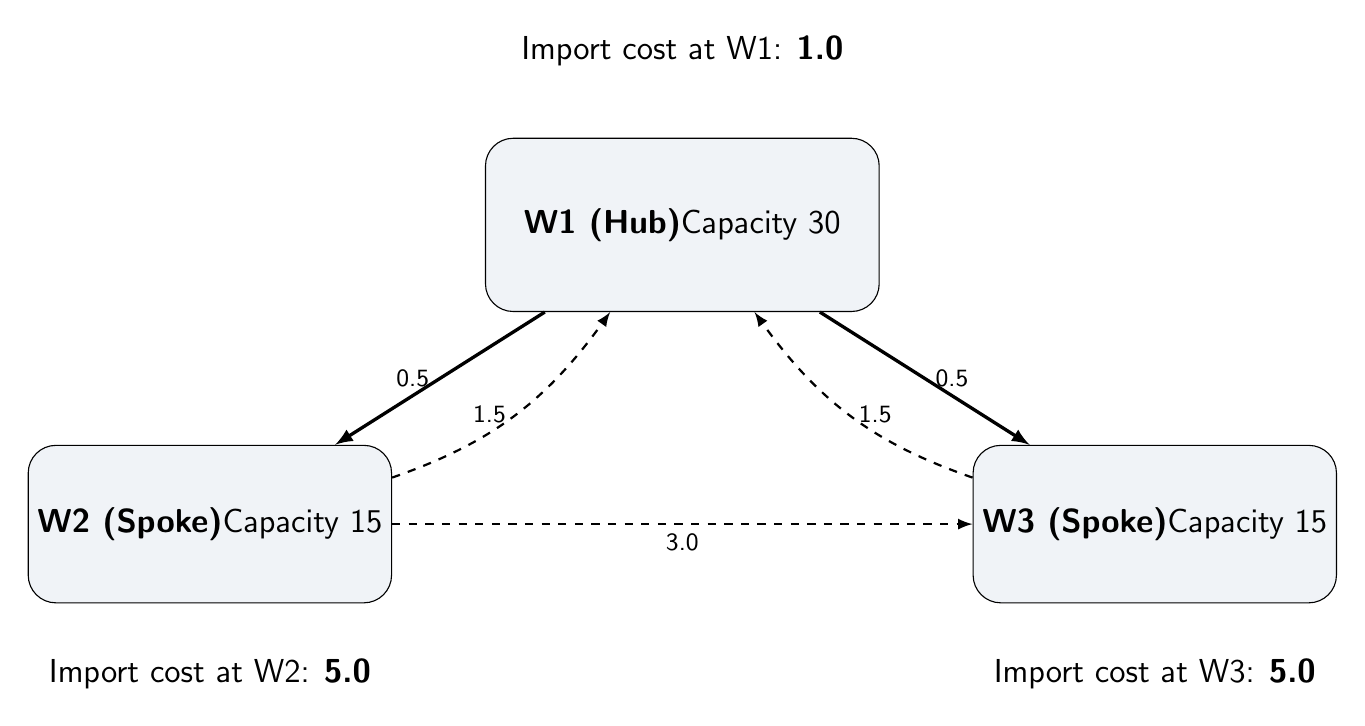
\begin{tikzpicture}[scale=1.0, every node/.style={font=\large}]
\node[draw, rounded corners=10pt, fill=PosterSoft, minimum width=5.0cm, minimum height=2.2cm] (w1) at (0,0) {\textbf{W1 (Hub)}\\Capacity 30};

\node[draw, rounded corners=10pt, fill=PosterSoft, minimum width=4.6cm, minimum height=2.0cm] (w2) at (-6.0,-3.8) {\textbf{W2 (Spoke)}\\Capacity 15};
\node[draw, rounded corners=10pt, fill=PosterSoft, minimum width=4.6cm, minimum height=2.0cm] (w3) at (6.0,-3.8) {\textbf{W3 (Spoke)}\\Capacity 15};

\draw[-latex, very thick] (w1) -- node[left] {\small 0.5} (w2);
\draw[-latex, very thick] (w1) -- node[right] {\small 0.5} (w3);
\draw[-latex, thick, dashed] (w2) -- node[below] {\small 3.0} (w3);
\draw[-latex, thick, dashed] (w3) to[bend left=18] node[right] {\small 1.5} (w1);
\draw[-latex, thick, dashed] (w2) to[bend right=18] node[left] {\small 1.5} (w1);

\node at (0,2.2) {\large Import cost at W1: \textbf{1.0}};
\node at (-6.0,-5.7) {\large Import cost at W2: \textbf{5.0}};
\node at (6.0,-5.7) {\large Import cost at W3: \textbf{5.0}};
\end{tikzpicture}

\smallskip
\small \textit{Hub-and-spoke warehouse network with cheaper replenishment at the hub and asymmetric transfer costs.}
\end{center}
}

\block[titleleft,roundedcorners=16]{2. Environment Design}{
\raggedright
\textbf{Warehouses and costs}

\begin{center}
\begin{tabular}{lcccc}
\toprule
Warehouse & Role & Cap. & Import & Hold. \\
\midrule
W1 & Hub   & 30 & 1.0 & 0.3 \\
W2 & Spoke & 15 & 5.0 & 1.0 \\
W3 & Spoke & 15 & 5.0 & 1.0 \\
\bottomrule
\end{tabular}
\hspace{1.2cm}
\begin{tabular}{lc}
\toprule
Transfer & Cost \\
\midrule
W1 $\to$ W2 / W3 & 0.5 \\
W2 / W3 $\to$ W1 & 1.5 \\
W2 $\leftrightarrow$ W3 & 3.0 \\
\bottomrule
\end{tabular}
\end{center}

\textbf{State}
\[
s=(\text{stock}_1,\text{stock}_2,\text{stock}_3,\text{month})
\]

\textbf{Demand}
\[
D_i(m)\sim \mathrm{Poisson}(\mu_i(m))
\]
\[
\mu_i(m)=\max\!\left(1,\;\text{base}_i+\text{amplitude}_i
\sin\!\left(\frac{2\pi(m-\text{phase}_i)}{12}\right)\right)
\]



\begin{center}
\includegraphics[width=0.82\linewidth]{demand_visualization.png}

\smallskip
\small \textit{Seasonal demand profile and sampled monthly demand realizations.}
\end{center}

\textbf{Action space}

\small
\begin{itemize}
\item \textbf{34 discrete actions} combining imports and optional transfers.

\end{itemize}

\begin{center}
\small
\begin{tabular}{lc}
\toprule
Action type & Count \\
\midrule
No-op & 1 \\
Single imports & 9 \\
Transfer-only & 12 \\
Bulk imports & 2 \\
Hub import + transfer & 6 \\
Hub-specific large actions & 4 \\
\bottomrule
\end{tabular}
\end{center}
}
\block[titleleft,roundedcorners=16]{3. Decision Process \& Reward}{
\raggedright
At each month, the controller:
\begin{enumerate}
\item applies imports,
\item applies transfers,
\item samples demand,
\item fulfills demand,
\item updates inventory,
\item computes the reward.
\end{enumerate}

\textbf{Reward}
\[
\begin{aligned}
R_t={}&-10\sum_i \text{unmet}_i-\sum_i c_i^{\mathrm{import}}\text{import}_i-\sum_{i,j} c_{ij}^{\mathrm{transfer}}\text{transfer}_{ij}\\
&-\sum_i c_i^{\mathrm{hold}}\text{stock}_i' - \text{infeasible units}
\end{aligned}
\]
\begin{itemize}
\item Unmet demand is heavily penalized to prioritize service level.
\item Imports and transfers contribute directly to operational cost.
\item Holding cost discourages unnecessary overstocking.
\item Infeasible actions are clamped and penalized.
\end{itemize}

\textbf{Episode setup}
\begin{itemize}
\item Horizon: \textbf{12 months}, Initial stock: \textbf{(15, 7, 7)} ,Discount factor: \textbf{$\gamma=0.95$}.
\end{itemize}
}

% =================================================
% CENTER COLUMN
% =================================================
\column{0.34}

\block[titleleft,roundedcorners=16]{4. Methods Compared}{
\raggedright
We compare \textbf{five discrete controllers} under the same 12-step seasonal environment.

\begin{itemize}
\item \textbf{Random}: uniform action selection over the 34 actions.
\item \textbf{Heuristic}: hand-crafted hub-first controller.
\item \textbf{Value Iteration}: finite-horizon planning,
\[
V_t(s)=\max_a \mathbb{E}\big[R(s,a,D)+\gamma V_{t+1}(s')\big],
\]
with stock coarsening step \textbf{4}.
\item \textbf{Q-Learning} and \textbf{SARSA}: tabular TD control with stock coarsening step \textbf{2}, $\alpha=0.1$, $\gamma=0.95$, and $\varepsilon$-greedy exploration from \textbf{1.0} to \textbf{0.05}.
\item \textbf{DQN}: neural approximation $Q(s,a)\approx Q_\theta(s,a)$ with 6 inputs, two hidden layers of size 64, and 34 outputs.
\end{itemize}

\begin{center}
\begin{tabular}{lccc}
\toprule
\small
Method & Type & State rep. & Main idea \\
\midrule
Random & baseline & exact & no learning \\
Heuristic & rules & exact & hub-first control \\
Value Iteration & planning & step-4 & finite-horizon DP \\
Q-Lear./ SARSA & tabular RL & step-2 & TD updates \\
DQN & deep RL & normalized & function approx. \\
\bottomrule
\end{tabular}
\end{center}

\textbf{Protocol}
\begin{itemize}
\item Value Iteration is solved by backward induction on the coarsened state space.
\item Q-Learning, SARSA, and DQN are trained for \textbf{50{,}000 episodes}.
\item Final policies are evaluated over \textbf{200 episodes}.
\item Main metrics: reward, unmet demand, service level, imports, transfers, and infeasible actions.
\end{itemize}

\textbf{Goal.} A good policy should both improve reward and recover the intended rule:
\[
\textbf{import at W1, then redistribute to W2 and W3.}
\]
}

\block[titleleft,roundedcorners=16]{5. Discrete Results}{
\raggedright
\begin{center}
\includegraphics[width=0.91\linewidth]{comparison_bars.png}

\smallskip
\small \textit{Discrete-method comparison on reward, service level, unmet demand, imports, transfers, and infeasible actions.}
\end{center}

\begin{center}
\begin{tabular}{lccc}
\toprule
Method & Avg reward & Service (\%) & Unmet \\
\midrule
Random & -1416.75 & 34.0 & 127.25 \\
Heuristic & -977.21 & 55.2 & 86.28 \\
Value Iteration & -735.44 & \textbf{72.1} & \textbf{54.04} \\
SARSA & -841.07 & 66.7 & 64.34 \\
DQN & \textbf{-732.65} & 71.2 & 55.85 \\
\bottomrule
\end{tabular}
\end{center}

\begin{itemize}
\item \textbf{DQN} gives the best average reward: \textbf{-732.65}.
\item \textbf{Value Iteration} gives the best service level: \textbf{72.1\%}.
\item \textbf{SARSA} improves over tabular Q-Learning on reward, unmet demand, and feasibility.
\item All informed methods drive infeasible actions close to zero, unlike the random baseline.
\end{itemize}
}

\block[titleleft,roundedcorners=16]{6. Hub Strategy \& Takeaway}{
\raggedright
\begin{center}
\includegraphics[width=0.91\linewidth]{combined_learning_curve.png}

\smallskip
\small \textit{Learning curves for Q-Learning, SARSA, and DQN against the main baselines.}
\end{center}

\begin{center}
\includegraphics[width=0.91\linewidth]{warehouse_transfer_breakdown.png}

\smallskip
\small \textit{Warehouse-level imports and transfers show whether a policy learned the hub-and-spoke structure.}
\end{center}

% \begin{itemize}
% \item Random stays far below all informed methods, while the heuristic is a strong non-learning baseline.
% \item \textbf{Value Iteration} and \textbf{DQN} learn the cleanest hub-centered flow pattern.
% \item \textbf{SARSA} is more stable than tabular Q-Learning and finishes with better reward and service.
% \item For \textbf{DQN}, almost all imports are centralized at \textbf{W1} (\textbf{109.7} units on average), while spoke imports are nearly zero.
% \item \textbf{Q-Learning} and \textbf{SARSA} recover the same logic less cleanly and still use spoke imports more often.

% \textbf{Discrete takeaway.}\\
% The strongest discrete policies are not only good on reward; they are also \textbf{interpretable}. The best controllers learn the intended operational structure instead of relying on unrealistic spoke imports.
}

% =================================================
% RIGHT COLUMN
% =================================================
\column{0.33}

\block[titleleft,roundedcorners=16]{7. Continuous Extension}{
\raggedright
\small
We extend to a \textbf{continuous-action} setting where the policy directly outputs shipment magnitudes between warehouses, instead of choosing from a fixed discrete list.

\begin{itemize}
\item For $N=4$ warehouses, the action is a transfer matrix $T\in\mathbb{R}^{N\times N}$: \textbf{16 continuous values}, one per directed pair.
\item The environment enforces feasibility: negatives are clipped to 0, the diagonal is zeroed, and rows exceeding available inventory are rescaled.
\item The cost matrix follows a hub-and-spoke topology — 1 hub, 3 spokes. Hub routes are cheapest; direct spoke-to-spoke transfers are most expensive.
\end{itemize}

\textbf{Reward}
\[
R_t = -C_{\text{transport}} - \lambda_d \sum_i U_i - C_{\text{overflow}}
\]
where $C_{\text{transport}}=\sum_{ij}c_{ij}T_{ij}$, $U_i=\max(0,D_i-I_i^{\text{post}})$ is unmet demand, and $\lambda_d=20$ makes service level the dominant signal.
}

\block[titleleft,roundedcorners=16]{8. PPO for Continuous Control}{
\raggedright
\small
PPO handles Gaussian continuous policies and keeps updates stable via the clipped surrogate:
\[
L^{\text{CLIP}}(\theta)=\hat{\mathbb{E}}_t\!\left[\min\!\Big(
\rho_t(\theta)\hat{A}_t,\;
\text{clip}(\rho_t(\theta),1{-}\varepsilon,1{+}\varepsilon)\hat{A}_t
\Big)\right]
\]
\textbf{Settings:} 14 parallel environments, 50 steps per rollout, 10 epochs, batch 256, lr $3\!\times\!10^{-4}$, $\gamma{=}0.99$, $\lambda_{\text{GAE}}{=}0.95$, network $[128,128]$.

\begin{center}
\small
\begin{tabular}{lcp{5.5cm}}
\toprule
Parameter & Value & Role \\
\midrule
\texttt{clip\_range} & $0.2\to0.0$ & Large updates early (explore), small updates late (exploit) \\
\texttt{log\_std\_init} & $-1.0$ & Initial std $\approx0.37$; default 1.0 causes excessive noise \\
\bottomrule
\end{tabular}
\end{center}

\textbf{Why we dropped the entropy bonus.}
High variance inflates actions to near-zero shipping; clip-range schedule explores more stably.

\textbf{Limitation \& future work.}
Stochastic demand makes credit assignment hard: a good shipping decision may still yield unmet demand by chance. Future work could incorporate demand forecasting or a GNN policy with explicit hub-spoke structure to close the remaining gap.
}

\block[titleleft,roundedcorners=16]{9. Continuous Results}{
\raggedright
\small

\begin{center}
\begin{tabular}{lccc}
\toprule
Agent & Demand sat.\ (\%) & Transport cost & Reward \\
\midrule
Random   & $\sim$30 & High          & $\sim{-}60{,}000$ \\
Greedy   & $\sim$74 & $\sim$6{,}000 & $\sim{-}42{,}000$ \\
PPO (2M) & \textbf{78}  & $\sim$\textbf{10}   & $\sim{-}7{,}000$  \\
\bottomrule
\end{tabular}
\end{center}

\begin{center}
\fbox{\parbox[c][6.5cm][c]{0.88\linewidth}{\centering\Large Learning Curves \& Flow Graph\\[0.6em]\normalsize Placeholder for PPO reward / satisfaction curves and transfer graph}}
\end{center}

\begin{itemize}
\item PPO matches the greedy heuristic on service level (\textbf{78\%}) while reaching near-\textbf{zero transport cost} --- the policy discovers cheap hub-routed redistribution.
\item The remaining gap to 100\% is driven by stochastic demand: with Poisson arrivals and finite inventory, some unmet demand is unavoidable regardless of the shipping strategy.
\end{itemize}
}

\end{columns}
\end{document}  
